\section{Bolzen- und Stiftverbindungen}
\subsection{Stiftverbindungen}
\begin{figure}[H]
	\centering
	\begin{minipage}[b]{0.22\linewidth}
		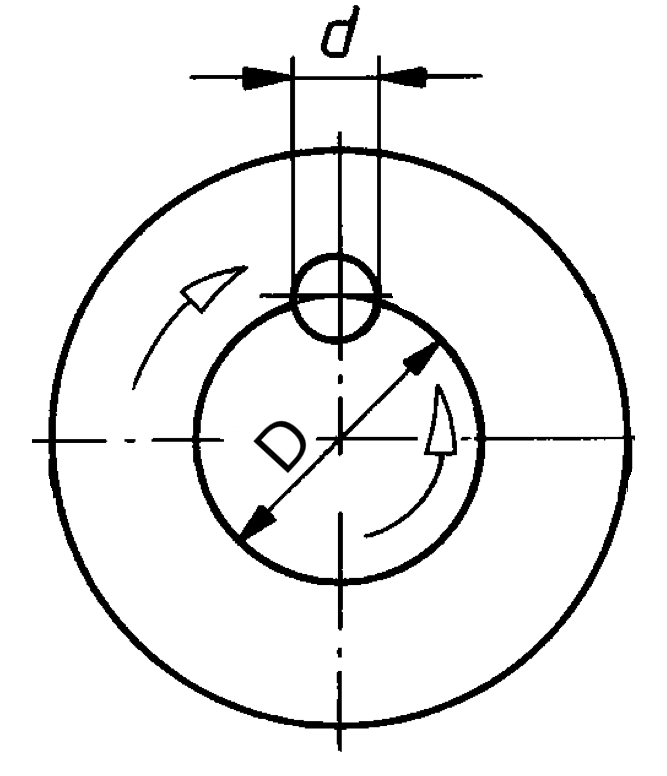
\includegraphics[width=\linewidth]{bolzen-und-stiftverbindungen/laengststift}
		\caption*{Längsstift}
	\end{minipage}
	\begin{minipage}[b]{0.22\linewidth}
		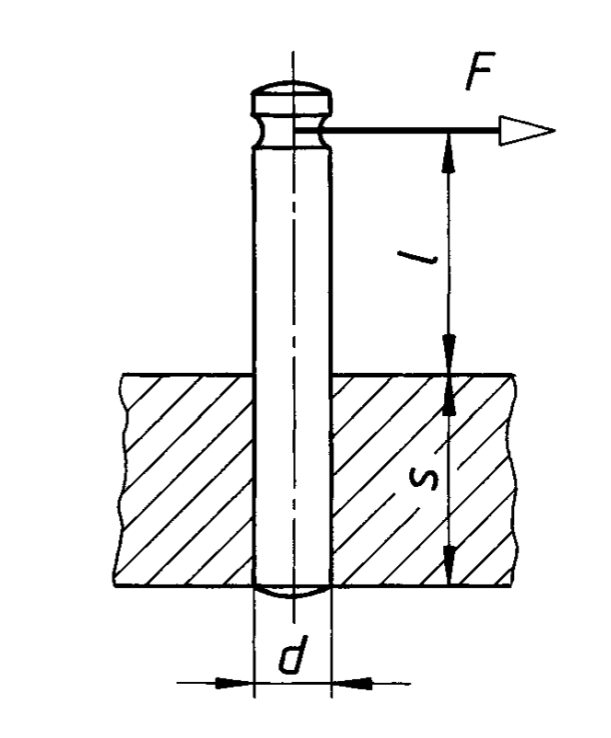
\includegraphics[width=\linewidth]{bolzen-und-stiftverbindungen/steckstift}
		\caption*{Steckstift}
	\end{minipage}
	\begin{minipage}[b]{0.22\linewidth}
		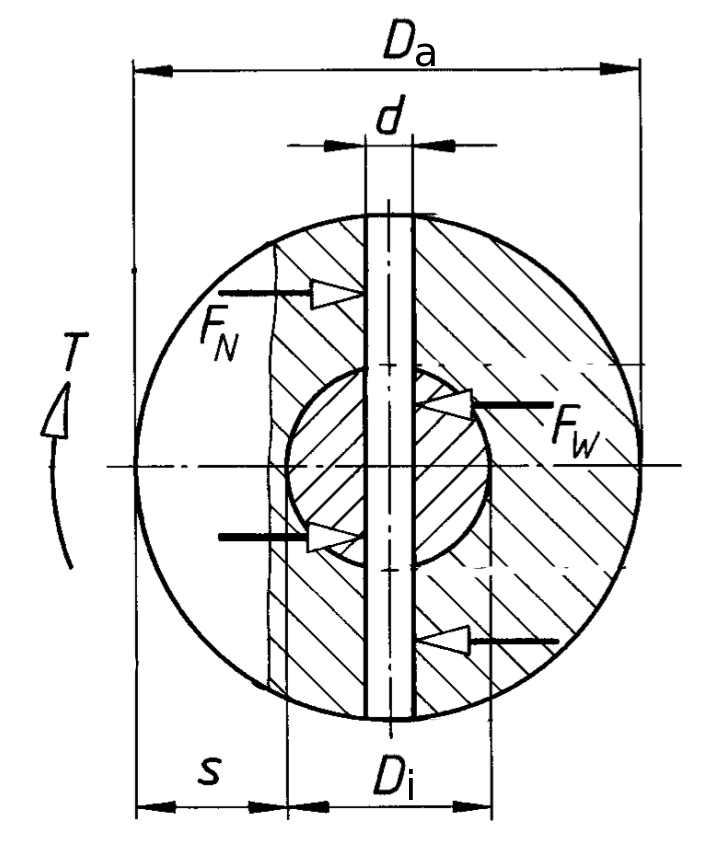
\includegraphics[width=\linewidth]{bolzen-und-stiftverbindungen/querstift}
		\caption*{Querstift}
	\end{minipage}
\end{figure}

% Längststiftverbindungen
\begin{eeqn}{Längsstiftverbindung}
	\begin{align}
		& P = \frac{4\cdot M}{L \cdot D \cdot d}\\
		& \tau_\text{A} = \frac{2\cdot M}{L \cdot D \cdot d}
	\end{align}
\end{eeqn}

% Steckstiftverbindung
\begin{eeqn}{Steckstiftverbindung}
	\begin{align}
		P_\text{max} &= \frac{2\cdot F}{d \cdot s}\cdot \left(3 \cdot \frac{l}{s}+2\right) + P_\text{Montage}
	\end{align}
	Maximale Pressung einer Steckstiftverbindung, die im Sitz zu erwarten ist. \\
	Beanspruchung des Stifts:
	\begin{align}
		&\tau_\text{A} = \frac{F}{A} = \frac{4\cdot F}{\pi \cdot d^2}\\
		&\sigma_\text{B} = \frac{M_\text{B}}{W_\text{ax}} = \frac{32\cdot F \cdot l}{\pi \cdot d^3}
 	\end{align}
 	Wenn beide Enden des Steckstifts versenkt sind, gilt (siehe Aufgabe 44):

	\begin{align}
		P &= \frac{F}{d\cdot s} \\
		\sigma_\text{B} &= \frac{M_\text{B}}{W_\text{ax}} = \frac{32\cdot F \cdot s}{\pi \cdot d^3 \cdot 2}
	\end{align}
\end{eeqn}



% Querstiftsverbindung
\begin{eeqn}{Querstiftsverbindung}
	Wenn auf die Welle das Moment $M$ wirkt, entsteht in der Narbe die Pressung $P_\text{N}$ und in der Welle die Pressung $P_\text{W}$:
	\begin{align}
		& P_\text{N} = \frac{4\cdot M}{d\cdot(D_\text{a}^2-D_\text{i}^2)} \\
		& P_\text{W} = \frac{6\cdot M}{d \cdot D_\text{i}^2}
	\end{align}
	Der Stift erleidet Scherspannungen:
	\begin{align}
		\tau_\text{A} &= \frac{4\cdot M}{\pi \cdot d^2 \cdot D_\text{i}}
	\end{align}
\end{eeqn}

\subsection{Bolzenverbindungen}
\begin{figure}[H]
	\centering
	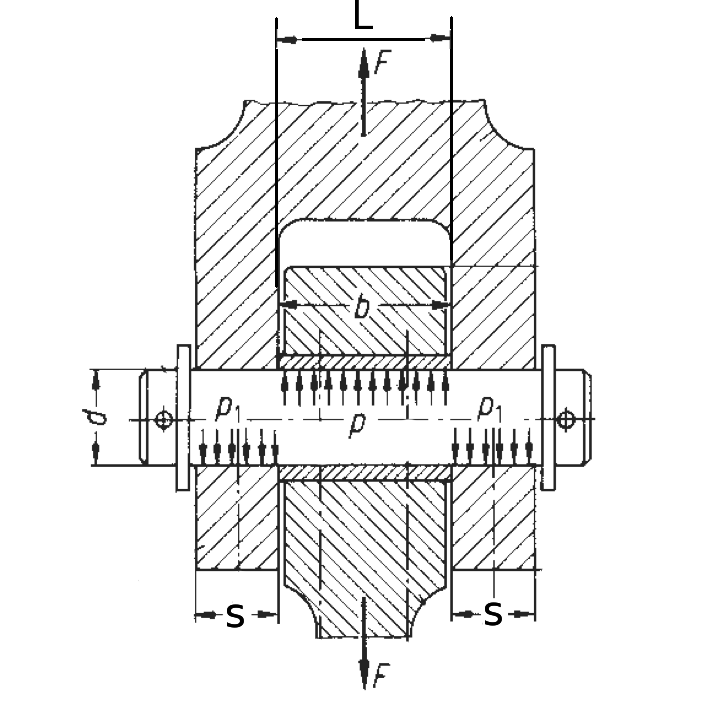
\includegraphics[width=0.7\linewidth]{bolzen-und-stiftverbindungen/bolzen}
	\caption*{Gabel-Welle Verbindung mit einem Bolzen}
\end{figure}
\vfill
\pagebreak
\hrule
% Biegemomente in Gabel Stange Verbindungen
\begin{eeqn}{Biegemomente in Gabel-Stange Verbindungen}
	\begin{table}[H]
		\centering
		\caption*{Unterschiedliche Passungsverhältnisse für Gabel-Stange Verbindungen}
		\begin{tabularx}{\linewidth}{llX}
			\toprule
			Passung Gabel & Passung Stange & $M_\text{B}$ \\
			\midrule
			Spiel & Spiel & $\displaystyle\frac{F\cdot (L+2\cdot s)}{8}$ \\[3mm]
			Pressung & Spiel & $\displaystyle\frac{F \cdot L}{8} $ \\[3mm]
			Spiel & Pressung & $\displaystyle\frac{F\cdot s}{4} $ \\
			\bottomrule
		\end{tabularx}
	\end{table}
\end{eeqn}

\begin{eeqn}{Gabel-Stange Verbindung}
	Zwischen Bolzen und Stange wirkt die Pressung $P_\text{Stange}$:
	\begin{align}
		P_\text{Stange} &= \frac{F}{L\cdot d}
	\end{align}
	Zwischen Bolzen und Gabel wirkt die Pressung $P_\text{Gabel}$:
	\begin{align}
		P_\text{Gabel} &= \frac{F}{2 \cdot s \cdot d}
	\end{align}
	Die Montagepressung $P_\text{Montage}$ wird beim auf Pressung beanspruchtem Element addiert.
	Der Bolzen erleidet Scher- und Biegespannungen:
	\begin{align}
		& \tau_\text{A} = \frac{2\cdot F}{\pi \cdot d^2} \\
		& \sigma_\text{B} = \frac{32\cdot M_\text{B}}{\pi \cdot d^3}
	\end{align}
\end{eeqn}

% Beanspruchung der Gabel
\begin{eeqn}{Beanspruchung der Gabel}
	Wenn auf einen Bolzen, der in einer Gabel gelagert ist, eine radiale Betriebskraft $F$ wirkt, entsteht in der Gabel eine Zugbeanspruchung $\sigma_\text{z}$:
	\begin{align}
		\sigma_\text{z} &= \frac{F}{A} = \frac{F}{2\cdot s\cdot (D-d)}
	\end{align}
	Hierbei hat die Gabel den Durchmesser $D$ und eine Dicke $s$. Der Bolzen hat den Durchmesser $d$. 
\end{eeqn}